\documentclass[a4paper,final]{article}
\usepackage[14pt]{extsizes}
\usepackage[T2A]{fontenc}
\usepackage[utf8]{inputenc}
\usepackage[russian]{babel}




\usepackage{amsmath}
\usepackage[left=20mm, top=20mm, right=20mm, bottom=20mm, footskip=10mm]{geometry}
\usepackage{ragged2e}
\usepackage{setspace}
\usepackage{alltt}
\usepackage{wrapfig}
\usepackage{moreverb} %листинги
\usepackage{indentfirst} % для абзацного отступа
\renewcommand\verbatimtabsize{4\relax}
\renewcommand\listingoffset{0.2em} %отступ от номеров строк
\renewcommand{\arraystretch}{1.4} % высота строки
\usepackage[font=small, singlelinecheck=false, justification=raggedleft, format=plain, labelsep=period]{caption} %заголовок таблицы
\usepackage{listings}
\usepackage{xcolor} % цвета
\usepackage{hyperref}% для гиперссылок
\usepackage{enumitem} %для перечислений
\usepackage{nccmath}
\usepackage{tikz}
\usepackage{wrapfig}
\usepackage{listings}
\usepackage{float}
\usepackage{shadow}
\usepackage{longtable}
\usepackage{multirow}
\usepackage{makecell}
\usepackage{longtable}
\usepackage{tabularx}
\usepackage{seqsplit}
\usepackage{subcaption} % Для подрисунков

\hypersetup{colorlinks,
  allcolors=[RGB]{000 000 000}} %гиперссылки

\textheight=24cm
\textwidth=16cm
\oddsidemargin=0pt
\topmargin=-1.5cm
\parindent=24pt % отступ абзаца по горизонтали
\parskip=5pt % отступ абзаца по вертикали
\tolerance=2000 % терпимость
\flushbottom % выравнивание высоты
\addto\captionsrussian{\def\refname{Список использованной литературы}}
\usepackage{xcolor}

%New colors defined below
\definecolor{codegreen}{rgb}{0,0.6,0}
\definecolor{codegray}{rgb}{0.5,0.5,0.5}
\definecolor{codepurple}{rgb}{0.58,0,0.82}
\definecolor{backcolour}{rgb}{0.95,0.95,0.92}


\definecolor{apricot}{HTML}{FFF0DA}
\definecolor{mygreen}{rgb}{0,0.6,0}
\definecolor{string}{HTML}{B40000} % цвет строк в коде
\definecolor{comment}{HTML}{008000} % цвет комментариев в коде
\definecolor{keyword}{HTML}{1A00FF} % цвет ключевых слов в коде
\definecolor{morecomment}{HTML}{8000FF} % цвет include и других элементов в коде
\definecolor{captiontext}{HTML}{FFFFFF} % цвет текста заголовка в коде
\definecolor{captionbk}{HTML}{999999} % цвет фона заголовка в коде
\definecolor{bk}{HTML}{FFFFFF} % цвет фона в коде
\definecolor{frame}{HTML}{999999} % цвет рамки в коде
\definecolor{brackets}{HTML}{B40000} % цвет скобок в коде

\setlist[enumerate,itemize]{leftmargin=1.2cm}

% подгружаемые языки — подробнее в документации listings
\lstloadlanguages{C++}

\newcommand{\doublecline}[1]{\noalign{\vskip-0.5\arrayrulewidth}\cline{#1}\noalign{\vskip-0.5\arrayrulewidth}\cline{#1}}

\begin{document}
\lstset{
  inputencoding=utf8,
  language=C++, % Язык кода по умолчанию
  morekeywords={*,...}, % если хотите добавить ключевые слова, то добавляйте
  % Цвета
  keywordstyle=\color{keyword}\ttfamily\bfseries,
  %stringstyle=\color{string}\ttfamily,
  stringstyle=\ttfamily\color{red!50!brown},
  commentstyle=\color{comment}\ttfamily,
  morecomment=[l][\color{morecomment}]{\#},
  % Настройки отображения
  breaklines=true, % Перенос длинных строк
  basicstyle=\ttfamily\footnotesize, % Шрифт для отображения кода
  backgroundcolor=\color{bk}, % Цвет фона кода
  frame=lrb,xleftmargin=\fboxsep,xrightmargin=-\fboxsep, % Рамка, подогнанная к заголовку
  rulecolor=\color{frame}, % Цвет рамки
  tabsize=3, % Размер табуляции в пробелах
  % Настройка отображения номеров строк. Если не нужно, то удалите весь блок
  numbers=left, % Слева отображаются номера строк
  stepnumber=1, % Каждую строку нумеровать
  numbersep=5pt, % Отступ от кода
  numberstyle=\small\color{black}, % Стиль написания номеров строк
  % Для отображения русского языка
  extendedchars=true,
  literate=
  {→}{{\ensuremath{\rightarrow}}}1
  {ε}{{\ensuremath{\varepsilon}}}1
  {á}{{\'a}}1  {é}{{\'e}}1  {í}{{\'i}}1  {ó}{{\'o}}1  {ú}{{\'u}}1
  {Á}{{\'A}}1  {É}{{\'E}}1  {Í}{{\'I}}1  {Ó}{{\'O}}1  {Ú}{{\'U}}1
  {ñ}{{\~n}}1  {Ñ}{{\~N}}1  {¿}{{{\textquestiondown}}}1  {¡}{{{\textexclamdown}}}1
  {Ö}{ {\''O} }1
  {~}{ {\textasciitilde} }1
  {а}{ {\selectfont\char224} }1
  {б}{ {\selectfont\char225} }1
  {в}{ {\selectfont\char226} }1
  {г}{ {\selectfont\char227} }1
  {д}{ {\selectfont\char228} }1
  {е}{ {\selectfont\char229} }1
  {ё}{ {\''e} }1
  {ж}{ {\selectfont\char230} }1
  {з}{ {\selectfont\char231} }1
  {и}{ {\selectfont\char232} }1
  {й}{ {\selectfont\char233} }1
  {к}{ {\selectfont\char234} }1
  {л}{ {\selectfont\char235} }1
  {м}{ {\selectfont\char236} }1
  {н}{ {\selectfont\char237} }1
  {о}{ {\selectfont\char238} }1
  {п}{ {\selectfont\char239} }1
  {р}{ {\selectfont\char240} }1
  {с}{ {\selectfont\char241} }1
  {т}{ {\selectfont\char242} }1
  {у}{ {\selectfont\char243} }1
  {ф}{ {\selectfont\char244} }1
  {х}{ {\selectfont\char245} }1
  {ц}{ {\selectfont\char246} }1
  {ч}{ {\selectfont\char247} }1
  {ш}{ {\selectfont\char248} }1
  {щ}{ {\selectfont\char249} }1
  {ъ}{ {\selectfont\char250} }1
  {ы}{ {\selectfont\char251} }1
  {ь}{ {\selectfont\char252} }1
  {э}{ {\selectfont\char253} }1
  {ю}{ {\selectfont\char254} }1
  {я}{ {\selectfont\char255} }1
  {А}{ {\selectfont\char192} }1
  {Б}{ {\selectfont\char193} }1
  {В}{ {\selectfont\char194} }1
  {Г}{ {\selectfont\char195} }1
  {Д}{ {\selectfont\char196} }1
  {Е}{ {\selectfont\char197} }1
  {Ё}{ {\''E} }1
  {Ж}{ {\selectfont\char198} }1
  {З}{ {\selectfont\char199} }1
  {И}{ {\selectfont\char200} }1
  {Й}{ {\selectfont\char201} }1
  {К}{ {\selectfont\char202} }1
  {Л}{ {\selectfont\char203} }1
  {М}{ {\selectfont\char204} }1
  {Н}{ {\selectfont\char205} }1
  {О}{ {\selectfont\char206} }1
  {П}{ {\selectfont\char207} }1
  {Р}{ {\selectfont\char208} }1
  {С}{ {\selectfont\char209} }1
  {Т}{ {\selectfont\char210} }1
  {У}{ {\selectfont\char211} }1
  {Ф}{ {\selectfont\char212} }1
  {Х}{ {\selectfont\char213} }1
  {Ц}{ {\selectfont\char214} }1
  {Ч}{ {\selectfont\char215} }1
  {Ш}{ {\selectfont\char216} }1
  {Щ}{ {\selectfont\char217} }1
  {Ъ}{ {\selectfont\char218} }1
  {Ы}{ {\selectfont\char219} }1
  {Ь}{ {\selectfont\char220} }1
  {Э}{ {\selectfont\char221} }1
  {Ю}{ {\selectfont\char222} }1
  {Я}{ {\selectfont\char223} }1
  {\{}{ { {\color{brackets}\{} } }1 % Цвет скобок {
  {\} }{ { {\color{brackets}\} } } }1 % Цвет скобок }
}


\thispagestyle{empty}
\begin{center}
\hfill \break
\hfill \break
\normalsize{МИНИСТЕРСТВО НАУКИ И ВЫСШЕГО ОБРАЗОВАНИЯ РОССИЙСКОЙ ФЕДЕРАЦИИ\\
 федеральное государственное автономное образовательное учреждение высшего образования «Санкт-Петербургский политехнический университет Петра Великого»\\[10pt]}
\normalsize{Институт компьютерных наук и кибербезопасности}\\[10pt] 
\normalsize{Высшая школа технологий искусственного интеллекта}\\[10pt] 
\normalsize{Направление: 02.03.01 <<Математика и компьютерные науки>>}\\
\vspace{50pt}
{\large Математическая логика и теория формальных языков\\
Отчёт о выполнении лабораторной работы №3 \\
<<Построение контекстно-свободной грамматики подмножества естественного языка>>\\[1em]
Вариант 35}
\end{center}
 \vspace{70pt}
\small{ 
\begin{tabular}{lrrl}
\!\!\!Студент, & \hspace{2cm} & & \\
\!\!\!группа 5130201/30102 & \hspace{2cm} & \underline{\hspace{3cm}} & Путята М. А.  \\\\
\!\!\!Преподаватель & \hspace{2cm} & \underline{\hspace{3cm}} &  Востров А. В. \\\\
&&\hspace{5cm}
\end{tabular}
\begin{flushright}
<<\underline{\hspace{1cm}}>>\underline{\hspace{2.5cm}} 2026 г.
\end{flushright}
}

\hfill \break
\begin{center} \small{Санкт-Петербург, 2026} \end{center}


\newpage
\tableofcontents
\newpage

\section*{Введение}
\addcontentsline{toc}{section}{Введение}

В ходе выполнения данной лабораторной работы необходимо разработать контекстно-свободную грамматику для выбранного подмножества естественного языка. Для выполнения работы будет реализовано подмножество испанского языка, охватывающее простые предложения во времени Futuro de indicativo (будущее простое) в утвердительной, отрицательной и вопросительной формах.

Требуется, чтобы разрабатываемая программа могла как генерировать корректные предложения, соответствующие реализуемой КСГ, так и определять корректность введённых пользователем предложений.

Для выполнения поставленной задачи необходимо:
\begin{enumerate}
    \item Изучить правила построения предложений, склонения существительных и спряжения глаголов в будущем простом времени испанского языка.
    \item Выделить подмножество испанского языка будущего простого времени.
    \item Формально описать грамматику данного языка и времени.
    \item Составить БНФ для реализуемой контекстно-свободной грамматики.
    \item Написать программную реализацию для созданной контекстно-свободной грамматики.
    \item Создать инструменты для проверки корректности предложений и генерации корректных предложений.
\end{enumerate}

\newpage
\section{Описание грамматики Futuro de indicativo}


Испанское будущее простое время используется для описания действий, которые произойдут после момента речи. Оно характеризуется специфическими окончаниями, добавляемыми к инфинитиву глагола. Данные окончания обязательно должны соответствовать лицу и числу существительного. В таблице 1 представлены окончания для всех лиц и чисел подлежащего.

\begin{longtable}{|c|c|c|}
\caption{} \\
\hline
\textbf{Лицо} & \textbf{Единственное число} & \textbf{Множественное число} \\ \hline
\endfirsthead
\hline
\textbf{Лицо} & \textbf{Единственное число} & \textbf{Множественное число} \\ \hline
\endhead

\hline \multicolumn{3}{r}{{Продолжение на следующей странице}} \\
\endfoot

\hline
\endlastfoot

1-е (Я / Мы) & -é & -emos \\\hline
2-е (Ты / Вы) & -ás & -éis \\\hline
3-е (Он, Она / Они) & -á & -án \\\hline
\end{longtable}

Также следует отметить, что существительные и прилагательные также должны быть согласованы между собой, но в отличии от существительного и глагола, они согласуются по роду и числу, то есть в испанском языке различаются прилагательные множественного числа для разных родов. Например в связке с существительным мужского рода множественного числа прилагательное ''быстрые'' будет переводится как ''rápidos'', а для женского рода во множественном числе -- ''rápidas'', но также есть и прилагательные-исключения, которые для обоих родов имеют одинаковое написание -- ''grandes'', ''interesantes'', ''importantes'' и другие.

\subsection{Примеры использования}
Данная грамматика позволяет строить предложения, описывающие намерения или будущие события:
\begin{itemize}
    \item \textbf{Yo hablaré con el profesor mañana.} -- Я поговорю с учителем завтра.
    \item \textbf{Ellos comerán en el restaurante.} -- Они будут есть в ресторане.
\end{itemize}

\subsection{Формы предложений}
Из написанных ниже форм предложений видно, что подлежащее является необязательной частью предложения, так как род и лицо глагола полностью совпадают с родом и лицом существительного, поэтому зачастую предложения строятся без подлежащего.
\subsubsection{Утвердительные предложения}
Строятся по схеме: \textbf{[Подлежащее] + (Инфинитив + -é / -ás / -á / -emos / -éis / -án) / Неправильный глагол + [Дополнение / Определение / Обстоятельство] + .}

Пример: \textbf{Yo hablaré con el profesor mañana.}

\subsubsection{Отрицательные предложения}
Имеют ту же схему, что и утвердительные предложения, но имеют частицу ''no'' перед глаголом.

Строятся по схеме: \textbf{[Подлежащее] + no + (Инфинитив + -é / -ás / -á / -emos / -éis / -án) / Неправильный глагол + [Дополнение / Определение / Обстоятельство] + .}

Пример: \textbf{Tú no comerás el libro.}

\subsubsection{Вопросительные предложения}
Используют обрамляющие знаки \textbf{¿} и \textbf{?}, а также необязательные вопросительные слова в начале предложения.

Строятся по схеме: \textbf{¿ + [Вопросительное слово] + (Инфинитив + -é / -ás / -á / -emos / -éis / -án) / Неправильный глагол + [Подлежащее] + [Дополнение / Определение / Обстоятельство] + ?}

Пример: \textbf{¿Cuándo comerá el gato?}

\newpage
\section{Математическое описание}
\subsection{Формальные грамматики}
Формальная грамматика является способом описания формального языка и определяется как четвёрка объектов: 
$$G = (T, N, S, R)$$
Где:
\begin{itemize}
    \item $T$ -- конечное множество терминалов;
    \item $N$ -- конечное множество нетерминалов, причём $T \cap N = \emptyset$;
    \item $S \in N$ -- начальный нетерминал;
    \item $R$ -- конечное множество правил вида $\alpha \rightarrow \beta$.
\end{itemize}

Иерархия Хомского -- это классификация формальных грамматик, по которой они делятся на 4 класса по их условной сложности:
\begin{enumerate}[label=Класс \arabic*., start=0]
    \item Неограниченные грамматики, правила которых могут быть записаны в виде $\alpha \rightarrow \beta$, где $\alpha$ -- любая непустая цепочка, содержащая хотя бы один нетерминальный символ, а $\beta$ -- любая цепочка из символов алфавита.
    \item Контексно-зависимые грамматики, правила которых имеют вид $\alpha A\beta \rightarrow \alpha\gamma\beta$, где $\alpha, \beta \in \{T \cup N\}^*, ~A \in N$ и $\gamma \in \{T \cup N\}^+$.
    \item Контекстно-свободные грамматики, которые определяют контекстно-свободные языки. Правила таких грамматик могут быть записаны в виде $A \rightarrow \beta$, где $A \in N$ и $\beta \in \{T \cup N\}^+$.
    \item Автоматные грамматики, которые задают регулярные языки. Подразделяются на леволинейные грамматики, правила которых записываются в виде $A \rightarrow B\gamma$ или $A \rightarrow \gamma$, и праволинейные, правила которых имеют вид $A \rightarrow \gamma B$ или $A \rightarrow \gamma$, где $\gamma \in T$ и $A, B \in N$.
\end{enumerate}

Язык, который порождает грамматика G, определяется множеством терминальных цепочек, которые можно вывести из начального нетерминала.

\subsection{Формальное определение грамматики Futuro de indicativo}
Грамматика будущего простого времени испанского языка была определена как контекстно-свободная грамматика $G = (T, N, S, R)$, где:
\begin{itemize}
    \item $T$ = \{ ''.'', ''¿'', ''?'', ''no'', ''yo'', ''tú'', ''él'', ''ella'', ''usted'', ''nosotros'', ''nosotras'', ''vosotros'', ''vosotras'', ''ellos'', ''ellas'', ''ustedes'', ''el'', ''un'', ''este'', ''mi'', ''tu'', ''su'', ''nuestro'', ''vuestro'', ''todo'', ''poco'', ''mucho'', ''la'', ''una'', ''esta'', ''nuestra'', ''vuestra'', ''toda'', ''poca'', ''mucha'', ''los'', ''unos'', ''estos'', ''mis'', ''tus'', ''sus'', ''nuestros'', ''vuestros'', ''todos'', ''pocos'', ''muchos'', ''las'', ''unas'', ''estas'', ''nuestras'', ''vuestras'', ''todas'', ''pocas'', ''muchas'', ''libro'', ''coche'', ''tiempo'', ''año'', ''trabajo'', ''amigo'', ''profesor'', ''perro'', ''gato'', ''árbol'', ''probleма'', ''casa'', ''ciudad'', ''vida'', ''escuela'', ''amiga'', ''profesora'', ''mesa'', ''puerta'', ''flor'', ''noche'', ''mano'', ''libros'', ''coches'', ''tiempos'', ''años'', ''trabajos'', ''amigos'', ''profesores'', ''perros'', ''gatos'', ''árboles'', ''problemas'', ''casas'', ''ciudades'', ''vidas'', ''escuelas'', ''amigas'', ''profesoras'', ''mesas'', ''puertas'', ''flores'', ''noches'', ''manos'', ''bueno'', ''nuevo'', ''viejo'', ''pequeño'', ''hermoso'', ''grande'', ''interesante'', ''importante'', ''rojo'', ''rápido'', ''inteligente'', ''buena'', ''nueva'', ''vieja'', ''pequeña'', ''hermosa'', ''roja'', ''rápida'', ''buenos'', ''nuevos'', ''viejos'', ''pequeños'', ''hermosos'', ''grandes'', ''interesantes'', ''importantes'', ''rojos'', ''rápidos'', ''inteligentes'', ''buenas'', ''nuevas'', ''viejas'', ''pequeñas'', ''hermosas'', ''rojas'', ''rápidas'', ''que'', ''en'', ''a'', ''de'', ''con'', ''por'', ''para'', ''sin'', ''sobre'', ''desde'', ''hasta'', ''entre'', ''bajo'', ''é'', ''ás'', ''á'', ''emos'', ''éis'', ''án'', ''hablar'', ''comer'', ''vivir'', ''estudiar'', ''viajar'', ''escribir'', ''leer'', ''коррер'', ''correr'', ''abrir'', ''recibir'', ''cantar'', ''bailar'', ''trabajar'', ''tendr'', ''vendr'', ''saldr'', ''podr'', ''querr'', ''habr'', ''dir'', ''har'', ''sabr'', ''pondr'', ''valdr'', ''cabr'', ''lo'', ''la'', ''los'', ''las'', ''le'', ''les'', ''mañana'', ''pronto'', ''siempre'', ''nunca'', ''rápidamente'', ''bien'', ''mal'', ''aquí'', ''allí'', ''también'', ''probablemente'', ''seguramente'', ''quizás'', ''qué'', ''quién'', ''quiénes'', ''cuándo'', ''dónde'', ''adónde'', ''por qué'', ''cómo'', ''cuál'', ''cuáles'', ''cuánto'', ''cuánta'', ''cuántos'', ''cuántas'' \} -- множество терминальных символов.
    \item $N$ = \{ sentence, affirmative, negative, interrogative, subj\_1sg, subj\_2sg, subj\_3sg, subj\_1pl, subj\_2pl, subj\_3pl, noun\_phrase\_ms, noun\_phrase\_fs, noun\_phrase\_mp, noun\_phrase\_fp, det\_ms, det\_fs, det\_mp, det\_fp, noun\_ms, noun\_fs, noun\_mp, noun\_fp, adj\_ms, adj\_fs, adj\_mp, adj\_fp, postmod\_ms, postmod\_fs, postmod\_mp, postmod\_fp, prep\_phrase\_ms, prep\_phrase\_fs, prep\_phrase\_mp, prep\_phrase\_fp, relative\_clause, verb\_any, preposition, verb\_1sg, verb\_2sg, verb\_3sg, verb\_1pl, verb\_2pl, verb\_3pl, inf, regular\_inf, irregular\_base, complements, complement, direct\_object, indirect\_object, adverbial, question\_word \} -- множество нетерминальных символов.
    \item $S$ = sentence -- начальный символ грамматики.
    \item R -- множество правил вывода вида $A \rightarrow \beta$, где $A \in N$ и $\beta \in \{T \cup N\}^+$. Правила вывода представлены следующем разделе.
\end{itemize}

\subsubsection{Правила вывода}
\paragraph{Типы предложений}\mbox{}\par
\begin{lstlisting}
    <sentence> → <affirmative> | <negative> | <interrogative>
\end{lstlisting}

\paragraph{Утвердительные предложения}\mbox{}\par
\begin{lstlisting}
    <affirmative> → <subj_1sg_opt> <verb_1sg> <complements> "."
    <affirmative> → <subj_2sg_opt> <verb_2sg> <complements> "."
    <affirmative> → <subj_3sg_opt> <verb_3sg> <complements> "."
    <affirmative> → <subj_1pl_opt> <verb_1pl> <complements> "."
    <affirmative> → <subj_2pl_opt> <verb_2pl> <complements> "."
    <affirmative> → <subj_3pl_opt> <verb_3pl> <complements> "."
    
    <subj_1sg_opt> → <subj_1sg> | ε
    <subj_2sg_opt> → <subj_2sg> | ε
    <subj_3sg_opt> → <subj_3sg> | ε
    <subj_1pl_opt> → <subj_1pl> | ε
    <subj_2pl_opt> → <subj_2pl> | ε
    <subj_3pl_opt> → <subj_3pl> | ε
\end{lstlisting}

\paragraph{Отрицательные предложения}\mbox{}\par
\begin{lstlisting}
    <negative> → <subj_1sg_opt> "no" <verb_1sg> <complements> "."
    <negative> → <subj_2sg_opt> "no" <verb_2sg> <complements> "."
    <negative> → <subj_3sg_opt> "no" <verb_3sg> <complements> "."
    <negative> → <subj_1pl_opt> "no" <verb_1pl> <complements> "."
    <negative> → <subj_2pl_opt> "no" <verb_2pl> <complements> "."
    <negative> → <subj_3pl_opt> "no" <verb_3pl> <complements> "."
\end{lstlisting}

\paragraph{Вопросительные предложения}\mbox{}\par
\begin{lstlisting}
    <interrogative> → "¿" <qword_opt> <verb_1sg> <subj_1sg_opt> <complements> "?"
    <interrogative> → "¿" <qword_opt> <verb_2sg> <subj_2sg_opt> <complements> "?"
    <interrogative> → "¿" <qword_opt> <verb_3sg> <subj_3sg_opt> <complements> "?"
    <interrogative> → "¿" <qword_opt> <verb_1pl> <subj_1pl_opt> <complements> "?"
    <interrogative> → "¿" <qword_opt> <verb_2pl> <subj_2pl_opt> <complements> "?"
    <interrogative> → "¿" <qword_opt> <verb_3pl> <subj_3pl_opt> <complements> "?"
    
    <qword_opt> → <question_word> | ε
\end{lstlisting}

\paragraph{Подлежащие}\mbox{}\par
\begin{lstlisting}
    <subj_1sg> → "yo"
    <subj_2sg> → "tú"
    <subj_3sg> → "él" | "ella" | "usted" | <noun_phrase_ms> | <noun_phrase_fs>
    <subj_1pl> → "nosotros" | "nosotras"
    <subj_2pl> → "vosotros" | "vosotras"
    <subj_3pl> → "ellos" | "ellas" | "ustedes" | <noun_phrase_mp> | <noun_phrase_fp>
\end{lstlisting}

\paragraph{Именные группы}\mbox{}\par
\begin{lstlisting}
    <noun_phrase_ms> → <det_ms_opt> <adj_ms_seq> <noun_ms> <postmod_ms_seq>
    <noun_phrase_fs> → <det_fs_opt> <adj_fs_seq> <noun_fs> <postmod_fs_seq>
    <noun_phrase_mp> → <det_mp_opt> <adj_mp_seq> <noun_mp> <postmod_mp_seq>
    <noun_phrase_fp> → <det_fp_opt> <adj_fp_seq> <noun_fp> <postmod_fp_seq>
    
    <det_ms_opt> → <det_ms> | ε
    <det_fs_opt> → <det_fs> | ε
    <det_mp_opt> → <det_mp> | ε
    <det_fp_opt> → <det_fp> | ε
    
    <adj_ms_seq> → <adj_ms> <adj_ms_seq> | ε
    <adj_fs_seq> → <adj_fs> <adj_fs_seq> | ε
    <adj_mp_seq> → <adj_mp> <adj_mp_seq> | ε
    <adj_fp_seq> → <adj_fp> <adj_fp_seq> | ε
    
    <postmod_ms_seq> → <postmod_ms> <postmod_ms_seq> | ε
    <postmod_fs_seq> → <postmod_fs> <postmod_fs_seq> | ε
    <postmod_mp_seq> → <postmod_mp> <postmod_mp_seq> | ε
    <postmod_fp_seq> → <postmod_fp> <postmod_fp_seq> | ε
\end{lstlisting}

\paragraph{Определители, существительные, прилагательные}\mbox{}\par
\begin{lstlisting}
    <det_ms> → "el" | "un" | "este" | "mi" | "tu" | "su" | "nuestro" | "vuestro" | "todo" | "poco" | "mucho"
    <det_fs> → "la" | "una" | "esta" | "mi" | "tu" | "su" | "nuestra" | "vuestra" | "toda" | "poca" | "mucha"
    <det_mp> → "los" | "unos" | "estos" | "mis" | "tus" | "sus" | "nuestros" | "vuestros" | "todos" | "pocos" | "muchos"
    <det_fp> → "las" | "unas" | "estas" | "mis" | "tus" | "sus" | "nuestras" | "vuestras" | "todas" | "pocas" | "muchas"
    
    <noun_ms> → "libro" | "coche" | "tiempo" | "año" | "trabajo" | "amigo" | "profesor" | "perro" | "gato" | "árbol" | "problema"
    <noun_fs> → "casa" | "ciudad" | "vida" | "escuela" | "amiga" | "profesora" | "mesa" | "puerta" | "flor" | "noche" | "mano"
    <noun_mp> → "libros" | "coches" | "tiempos" | "años" | "trabajos" | "amigos" | "profesores" | "perros" | "gatos" | "árboles" | "problemas"
    <noun_fp> → "casas" | "ciudades" | "vidas" | "escuelas" | "amigas" | "profesoras" | "mesas" | "puertas" | "flores" | "noches" | "manos"
    
    <adj_ms> → "bueno" | "nuevo" | "viejo" | "pequeño" | "hermoso" | "grande" | "interesante" | "importante" | "rojo" | "rápido" | "inteligente"
    <adj_fs> → "buena" | "nueva" | "vieja" | "pequeña" | "hermosa" | "grande" | "interesante" | "importante" | "roja" | "rápida" | "inteligente"
    <adj_mp> → "buenos" | "nuevos" | "viejos" | "pequeños" | "hermosos" | "grandes" | "interesantes" | "importantes" | "rojos" | "rápidos" | "inteligentes"
    <adj_fp> → "buenas" | "nuevas" | "viejas" | "pequeñas" | "hermosas" | "grandes" | "interesantes" | "importantes" | "rojas" | "rápidas" | "inteligentes"
\end{lstlisting}

\paragraph{Постмодификаторы}\mbox{}\par
\begin{lstlisting}
    <postmod_ms> → <prep_phrase_ms> | <relative_clause>
    <postmod_fs> → <prep_phrase_fs> | <relative_clause>
    <postmod_mp> → <prep_phrase_mp> | <relative_clause>
    <postmod_fp> → <prep_phrase_fp> | <relative_clause>
    
    <prep_phrase_ms> → <preposition> <noun_phrase_ms>
    <prep_phrase_fs> → <preposition> <noun_phrase_fs>
    <prep_phrase_mp> → <preposition> <noun_phrase_mp>
    <prep_phrase_fp> → <preposition> <noun_phrase_fp>
    
    <relative_clause> → "que" <verb_any> <complements>
    <verb_any> → <verb_1sg> | <verb_2sg> | <verb_3sg> | <verb_1pl> | <verb_2pl> | <verb_3pl>
    <preposition> → "en" | "a" | "de" | "con" | "por" | "para" | "sin" | "sobre" | "desde" | "hasta" | "entre" | "bajo"
\end{lstlisting}

\paragraph{Глаголы}\mbox{}\par
\begin{lstlisting}
    <verb_1sg> → <inf> "é"
    <verb_2sg> → <inf> "ás"
    <verb_3sg> → <inf> "á"
    <verb_1pl> → <inf> "emos"
    <verb_2pl> → <inf> "éis"
    <verb_3pl> → <inf> "án"
    
    <inf> → <regular_inf> | <irregular_base>
    <regular_inf> → "hablar" | "comer" | "vivir" | "estudiar" | "viajar" | "escribir" | "leer" | "correr" | "abrir" | "recibir" | "cantar" | "bailar" | "trabajar"
    <irregular_base> → "tendr" | "vendr" | "saldr" | "podr" | "querr" | "habr" | "dir" | "har" | "sabr" | "pondr" | "valdr" | "cabr"
\end{lstlisting}

\paragraph{Дополнения и обстоятельства}\mbox{}\par
\begin{lstlisting}
    <complements> → <complement> <complements> | <complements> <complement> | ε
    <complement> → <direct_object> | <indirect_object> | <adverbial>
    
    <direct_object> → <noun_phrase_ms> | <noun_phrase_fs> | <noun_phrase_mp> | <noun_phrase_fp> | "lo" | "la" | "los" | "las"
    <indirect_object> → "a" <noun_phrase_ms> | "a" <noun_phrase_fs> | "a" <noun_phrase_mp> | "a" <noun_phrase_fp> | "le" | "les"
    
    <adverbial> → "mañana" | "pronto" | "siempre" | "nunca" | "rápidamente" | "bien" | "mal" | "aquí" | "allí" | "también" | "probablemente" | "seguramente" | "quizás"
\end{lstlisting}

\paragraph{Вопросительные слова}\mbox{}\par
\begin{lstlisting}
    <question_word> → "qué" | "quién" | "quiénes" | "cuándo" | "dónde" | "adónde" | "por qué" | "cómo" | "cuál" | "cuáles" | "cuánto" | "cuánta" | "cuántos" | "cuántas"
\end{lstlisting}

\subsubsection{Представление рассматриваемой грамматики в БНФ}

Форма Бэкуса-Наура (БНФ) -- форма для представления контекстно-свободных грамматик. В данной форме продукции имеющие одинаковые левые части объединены с помощью объединения правых частей через знак <<|>>.

Для БНФ также существуют расширения позволяющие добавлять регулярные конструкции такие как группировка (a | \{b\} | c), итерация \{a\} и опциональность [a].

На листинге 1 представлена грамматика подмножества испанского языка в будущем простом времени в расширенной БНФ.\\[3em]

\footnotesize{
\begin{lstlisting}[caption = {Грамматика подмножества языка в БНФ}]
<sentence> ::= <affirmative> | <negative> | <interrogative>

УТВЕРДИТЕЛЬНОЕ
<affirmative> ::= [<subj_1sg>] <verb_1sg> <complements> "."
| [<subj_2sg>] <verb_2sg> <complements> "."
| [<subj_3sg>] <verb_3sg> <complements> "."
| [<subj_1pl>] <verb_1pl> <complements> "."
| [<subj_2pl>] <verb_2pl> <complements> "."
| [<subj_3pl>] <verb_3pl> <complements> "."

ОТРИЦАТЕЛЬНОЕ
<negative> ::= [<subj_1sg>] "no" <verb_1sg> <complements> "."
| [<subj_2sg>] "no" <verb_2sg> <complements> "."
| [<subj_3sg>] "no" <verb_3sg> <complements> "."
| [<subj_1pl>] "no" <verb_1pl> <complements> "."
| [<subj_2pl>] "no" <verb_2pl> <complements> "."
| [<subj_3pl>] "no" <verb_3pl> <complements> "."

ВОПРОСИТЕЛЬНОЕ
<interrogative> ::= "¿" [<question_word>] <verb_1sg> [<subj_1sg>] <complements> "?"
| "¿" [<question_word>] <verb_2sg> [<subj_2sg>] <complements> "?"
| "¿" [<question_word>] <verb_3sg> [<subj_3sg>] <complements> "?"
| "¿" [<question_word>] <verb_1pl> [<subj_1pl>] <complements> "?"
| "¿" [<question_word>] <verb_2pl> [<subj_2pl>] <complements> "?"
| "¿" [<question_word>] <verb_3pl> [<subj_3pl>] <complements> "?"

ПОДЛЕЖАЩИЕ
<subj_1sg> ::= "yo"
<subj_2sg> ::= "tú"
<subj_3sg> ::= "él" | "ella" | "usted" | <noun_phrase_ms> | <noun_phrase_fs>
<subj_1pl> ::= "nosotros" | "nosotras"
<subj_2pl> ::= "vosotros" | "vosotras"
<subj_3pl> ::= "ellos" | "ellas" | "ustedes" | <noun_phrase_mp> | <noun_phrase_fp>
ИМЕННЫЕ ГРУППЫ
<noun_phrase_ms> ::= [<det_ms>] {<adj_ms>} <noun_ms> {<postmod_ms>}
<noun_phrase_fs> ::= [<det_fs>] {<adj_fs>} <noun_fs> {<postmod_fs>}
<noun_phrase_mp> ::= [<det_mp>] {<adj_mp>} <noun_mp> {<postmod_mp>}
<noun_phrase_fp> ::= [<det_fp>] {<adj_fp>} <noun_fp> {<postmod_fp>}

ОПРЕДЕЛИТЕЛИ
<det_ms> ::= "el" | "un" | "este" | "mi" | "tu" | "su" | "nuestro" | "vuestro" | "todo" | "poco" | "mucho"
<det_fs> ::= "la" | "una" | "esta" | "mi" | "tu" | "su" | "nuestra" | "vuestra" | "toda" | "poca" | "mucha"
<det_mp> ::= "los" | "unos" | "estos" | "mis" | "tus" | "sus" | "nuestros" | "vuestros" | "todos" | "pocos" | "muchos"
<det_fp> ::= "las" | "unas" | "estas" | "mis" | "tus" | "sus" | "nuestras" | "vuestras" | "todas" | "pocas" | "muchas"

СУЩЕСТВИТЕЛЬНЫЕ
<noun_ms> ::= "libro" | "coche" | "tiempo" | "año" | "trabajo" | "amigo" | "profesor" | "perro" | "gato" | "árbol" | "problema"
<noun_fs> ::= "casa" | "ciudad" | "vida" | "escuela" | "amiga" | "profesora" | "mesa" | "puerta" | "flor" | "noche" | "mano"
<noun_mp> ::= "libros" | "coches" | "tiempos" | "años" | "trabajos" | "amigos" | "profesores" | "perros" | "gatos" | "árboles" | "problemas"
<noun_fp> ::= "casas" | "ciudades" | "vidas" | "escuelas" | "amigas" | "profesoras" | "mesas" | "puertas" | "flores" | "noches" | "manos"

ПРИЛАГАТЕЛЬНЫЕ
<adj_ms> ::= "bueno" | "nuevo" | "viejo" | "pequeño" | "hermoso" | "grande" | "interesante" | "importante" | "rojo" | "rápido" | "inteligente"
<adj_fs> ::= "buena" | "nueva" | "vieja" | "pequeña" | "hermosa" | "grande" | "interesante" | "importante" | "roja" | "rápida" | "inteligente"
<adj_mp> ::= "buenos" | "nuevos" | "viejos" | "pequeños" | "hermosos" | "grandes" | "interesantes" | "importantes" | "rojos" | "rápidos" | "inteligentes"
<adj_fp> ::= "buenas" | "nuevas" | "viejas" | "pequeñas" | "hermosas" | "grandes" | "interesantes" | "importantes" | "rojas" | "rápidas" | "inteligentes"

ПОСТМОДИФИКАТОРЫ
<postmod_ms> ::= <prep_phrase_ms> | <relative_clause>
<postmod_fs> ::= <prep_phrase_fs> | <relative_clause>
<postmod_mp> ::= <prep_phrase_mp> | <relative_clause>
<postmod_fp> ::= <prep_phrase_fp> | <relative_clause>
<prep_phrase_ms> ::= <preposition> <noun_phrase_ms>
<prep_phrase_fs> ::= <preposition> <noun_phrase_fs>
<prep_phrase_mp> ::= <preposition> <noun_phrase_mp>
<prep_phrase_fp> ::= <preposition> <noun_phrase_fp>
<relative_clause> ::= "que" <verb_any> <complements>
<verb_any> ::= <verb_1sg> | <verb_2sg> | <verb_3sg> | <verb_1pl> | <verb_2pl> | <verb_3pl>
<preposition> ::= "en" | "a" | "de" | "con" | "por" | "para" | "sin" | "sobre" | "desde" | "hasta" | "entre" | "bajo"

ГЛАГОЛ В БУДУЩЕМ ПРОСТОМ
<verb_1sg> ::= <inf> "é"
<verb_2sg> ::= <inf> "ás"
<verb_3sg> ::= <inf> "á"
<verb_1pl> ::= <inf> "emos"
<verb_2pl> ::= <inf> "éis"
<verb_3pl> ::= <inf> "án"
<inf> ::= <regular_inf> | <irregular_base>
<regular_inf> ::= "hablar" | "comer" | "vivir" | "estudiar" | "viajar" | "escribir" | "leer" | "correr" | "abrir" | "recibir" | "cantar" | "bailar" | "trabajar"
<irregular_base> ::= "tendr" | "vendr" | "saldr" | "podr" | "querr" | "habr" | "dir" | "har" | "sabr" | "pondr" | "valdr" | "cabr"

ДОПОЛНЕНИЯ И ОБСТОЯТЕЛЬСТВА
<complements> ::= <complement> <complements> | <complements> <complement> | $\epsilon$
<complement> ::= <direct_object> | <indirect_object> | <adverbial>
<direct_object> ::= <noun_phrase_ms> | <noun_phrase_fs> | <noun_phrase_mp> | <noun_phrase_fp> | "lo" | "la" | "los" | "las"
<indirect_object> ::= "a" <noun_phrase_ms> | "a" <noun_phrase_fs> | "a" <noun_phrase_mp> | "a" <noun_phrase_fp> | "le" | "les"
<adverbial> ::= "mañana" | "pronto" | "siempre" | "nunca" | "rápidamente" | "bien" | "mal" | "aquí" | "allí" | "también" | "probablemente" | "seguramente" | "quizás"

ВОПРОСИТЕЛЬНЫЕ СЛОВА
<question_word> ::= "qué" | "quién" | "quiénes" | "cuándo" | "dónde" | "adónde" | "por qué" | "cómo" | "cuál" | "cuáles" | "cuánto" | "cuánta" | "cuántos" | "cuántas"
\end{lstlisting}
}
\small

\subsubsection{Примеры предложений описанной грамматики}
\begin{itemize}
    \item Утвердительные
    \begin{itemize}
        \item Hablaré aquí ciudades que leerán le.
        \item Nosotras no bailaremos allí roja amiga mañana.
    \end{itemize}
    \item Отрицательные
    \begin{itemize}
        \item Nosotras no bailaremos allí mañana.
        \item No leerás nuevas profesoras por sus rápidas ciudades.
    \end{itemize}
    \item Вопросительные
    \begin{itemize}
        \item ¿Cuántas bailaremos nosotras pronto?
        \item ¿Adónde sabréis vosotras a mi pequeño viejo libro?
    \end{itemize}
\end{itemize}

Данная грамматика не может быть упрощена до автоматной, так как:
\begin{itemize}
    \item в ней есть косвенная рекурсия:

    <noun\_phrase\_ms> ::= [<det\_ms>] \{ <adj\_ms>\} < noun\_ms > \{ <postmod\_ms>\}
    
    <postmod\_ms> ::= <prep\_phrase\_ms> | <relative\_clause>
    
    <prep\_phrase\_ms> ::= <preposition> <noun\_phrase\_ms>

    \item в ней есть двусторонняя рекурсия:

    <complements> ::= <complement> <complements> | <complements> <complement> | $\epsilon$
\end{itemize}

На рисунке 1 представлен пример дерева построения предложения по реализованной грамматике для предложения ''¿Cabremos a años los gatos probablemente mañana?''.




\begin{figure}[H]
    \centering
    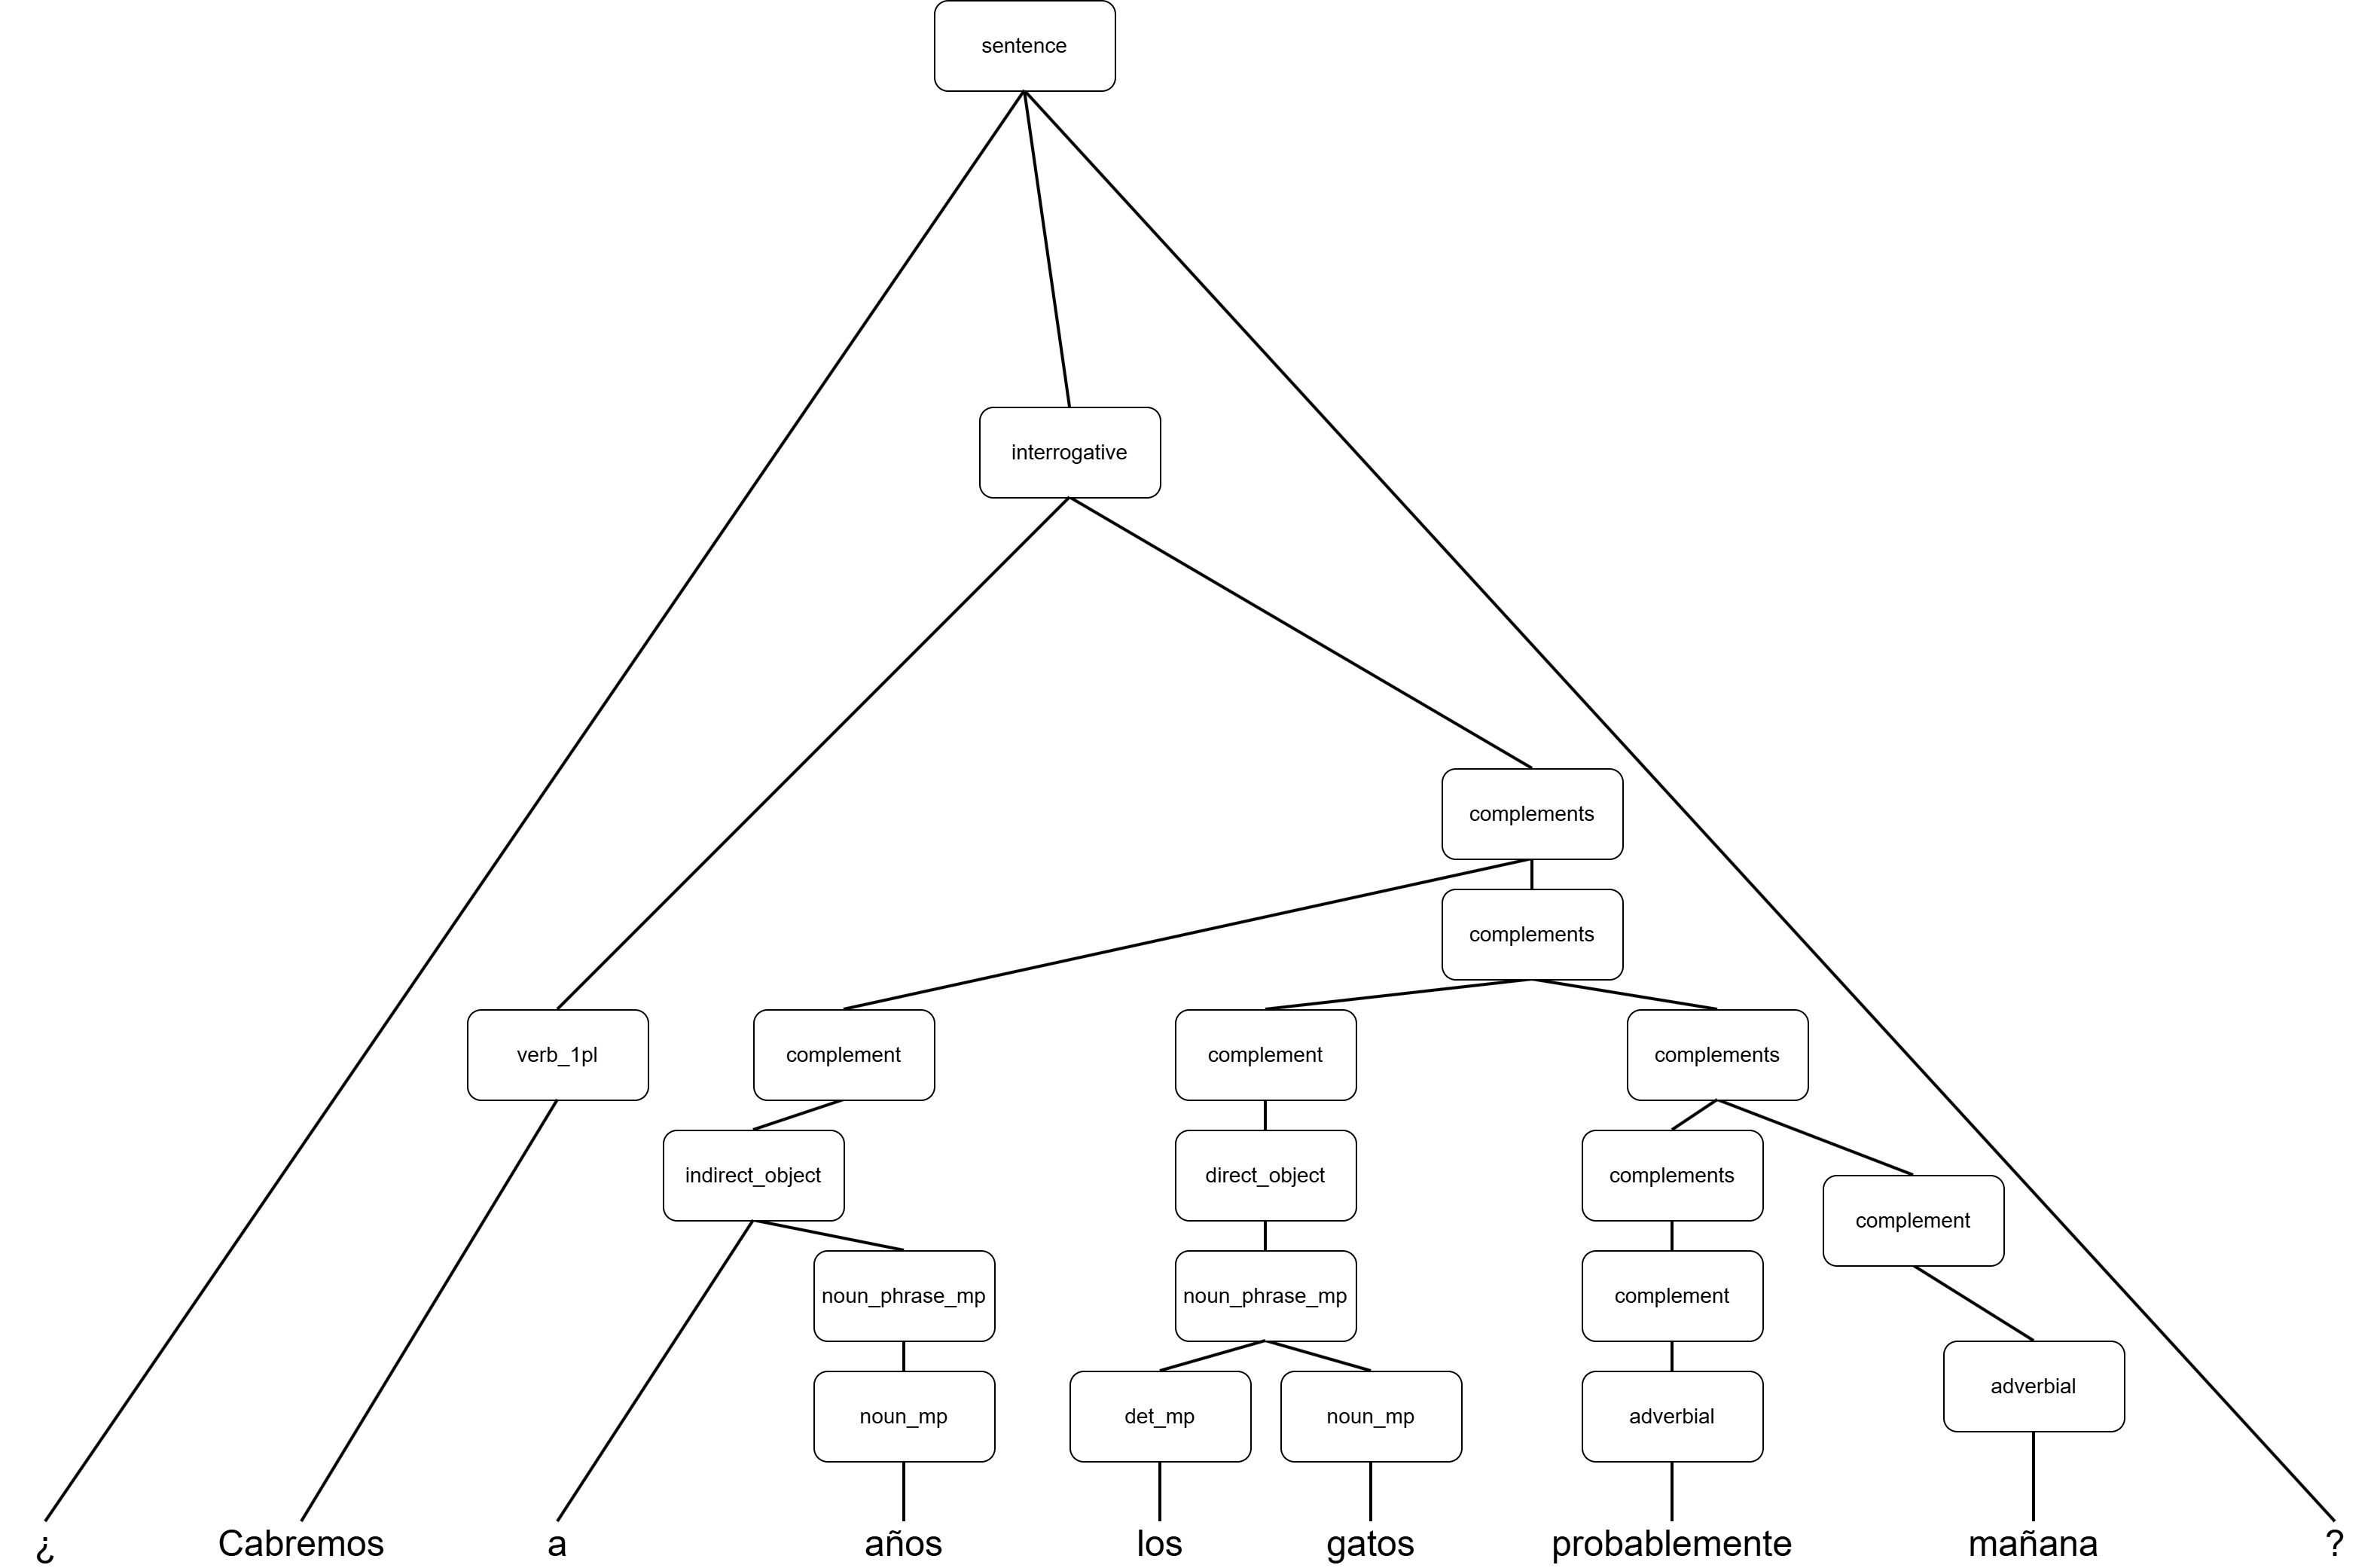
\includegraphics[width=1\linewidth]{разбор предложения.jpg}
    \caption{\centeringДерево построения предложения}
\end{figure}

\newpage
\section{Особенности реализации}

\subsection{Структура TreeNode}

Данная структура позволяет хранить узел N-арного дерева. Объекты этой структуры динамически создаются во время рекурсивного спуска в методе parseNode и parseErrorTree для формирования синтаксического дерева. В случае если ветка разбора оказывается тупиковой, узлы уничтожаются, иначе -- полученное дерево (экземпляр, представляющий корень) передаётся в функцию отрисовки дерева в консоли. На листинге 2 представлен код определения данной структуры.

\footnotesize{
\begin{lstlisting}[language=C++, caption = {Структура TreeNode}]
struct TreeNode {
	string symbol;
	vector<TreeNode*> children;

	TreeNode(string s) : symbol(s) {}

	~TreeNode() {
		for (auto c : children) {
			delete c;
		}
	}
};
\end{lstlisting}
}
\small

\paragraph{Назначение полей}
\begin{itemize}
    \item symbol -- строковое представление узла для вывода в консоль. Например, ''complements'' или ''noun\_phrase\_mp'';
    \item children -- вектор указателей на дочерние узлы дерева.
\end{itemize}

\subsection{Класс LanguageModel}
Данный класс реализует логику КС грамматики. Использование класса LanguageModel позволяет создавать грамматики для любых КС языков с помощью простого добавления правил вывода с помощью метода addRule. Класс объединяет в себе базу правил вывода, генератор предложений и синтаксический анализатор. Код определения данного класс представлен на листинге 3.
\footnotesize{
\begin{lstlisting}[language=C++, caption = {Класс LanguageModel}]
class LanguageModel {
private:
	Grammar rules;
	vector<string> vocabulary;
	size_t max_parse_pos = 0;

	void addRule(const string& l, const vector<vector<string>>& r) {
		rules[l] = r;
	}

	void buildGrammar();
	void generateNode(const string& symbol, vector<string>& output, int depth = 0);
	bool parseNode(const vector<string>& tokens, size_t& pos, const string& symbol, TreeNode*& out_node);
	int parseErrorTree(const vector<string>& tokens, size_t& pos, const string& symbol, TreeNode*& out_node);
	void replaceAll(string& str, const string& from, const string& to);
	void printTree(TreeNode* node, string prefix = "", bool isLast = true);
    
	bool isCapitalized(const string& str);
	string lowercaseUtf8(const string& str);
	string capitalizeUtf8(const string& str);

public:
	LanguageModel();

	string tokensToString(const vector<string>& tokens);
	vector<string> generateTokenList();
	void checkAndPrintSentence(string text, int tree_flag = 0);
};
\end{lstlisting}
}
\small

\paragraph{Назначение полей}
\begin{itemize}
    \item rules -- словарь, алфавит грамматики.
    \item vocabulary -- множество всех возможных терминалов заданного языка.
    \item max\_parse\_pos -- переменная, хранящая самый длинный индекс слова при разборе и использующаяся для возврата назад по предложению.
\end{itemize}

\paragraph{Конструктор класса}
Реализованный конструктор для данного класса используется для задания сида генерации случайных чисел и заполнения правил вывода экземпляра. Код конструктора представлен на листинге 4.

Вход: набор правил вывода и текущее время.

Выход: экземпляр класса LanguageModel.

\footnotesize{
\begin{lstlisting}[language=C++, caption = {Конструктор класса LanguageModel}]
LanguageModel() {
		srand((unsigned)time(0));
		buildGrammar();
	}
\end{lstlisting}
}
\small


\subsubsection{Метод buildGrammar}
Данный метод используется в конструкторе класса LanguageModel для задания правил вывода и формирования алфавита. buildGrammar содержит множественные вызовы метода addRule для определения каждого правила. Также для уменьшения размера исходного кода при определении правил вывода, содержащих терминалы глаголов, используется цикл, который формирует все возможные глаголы будущего времени с помощью комбинации каждого глагола с каждым возможным окончанием. На листинге 5 можно увидеть код данного метода.

Вход: набор правил вывода грамматики испанского языка.

Выход: заполненные правила вывода и алфавит класса LanguageModel.

\footnotesize{
\begin{lstlisting}[language=C++, caption = {Код метода buildGrammar}]
void buildGrammar() {
	addRule("subj_1sg", { {"yo"} });
	addRule("subj_2sg", { {"tú"} });
	addRule("subj_3sg", { {"él"}, {"ella"}, {"usted"}, {"noun_phrase_ms"}, {"noun_phrase_fs"} });
	addRule("subj_1pl", { {"nosotros"}, {"nosotras"} });
	addRule("subj_2pl", { {"vosotros"}, {"vosotras"} });
	addRule("subj_3pl", { {"ellos"}, {"ellas"}, {"ustedes"}, {"noun_phrase_mp"}, {"noun_phrase_fp"} });

	addRule("opt_subj_1sg", { {"subj_1sg"}, {} });
	addRule("opt_subj_2sg", { {"subj_2sg"}, {} });
	addRule("opt_subj_3sg", { {"subj_3sg"}, {} });
	addRule("opt_subj_1pl", { {"subj_1pl"}, {} });
	addRule("opt_subj_2pl", { {"subj_2pl"}, {} });
	addRule("opt_subj_3pl", { {"subj_3pl"}, {} });

	addRule("sentence", { {"affirmative"}, {"negative"}, {"interrogative"} });

	addRule("affirmative", {
		{"opt_subj_1sg", "verb_1sg", "complements", "."},
		{"opt_subj_2sg", "verb_2sg", "complements", "."},
		{"opt_subj_3sg", "verb_3sg", "complements", "."},
		{"opt_subj_1pl", "verb_1pl", "complements", "."},
		{"opt_subj_2pl", "verb_2pl", "complements", "."},
		{"opt_subj_3pl", "verb_3pl", "complements", "."}
		});

	addRule("negative", {
		{"opt_subj_1sg", "no", "verb_1sg", "complements", "."},
		{"opt_subj_2sg", "no", "verb_2sg", "complements", "."},
		{"opt_subj_3sg", "no", "verb_3sg", "complements", "."},
		{"opt_subj_1pl", "no", "verb_1pl", "complements", "."},
		{"opt_subj_2pl", "no", "verb_2pl", "complements", "."},
		{"opt_subj_3pl", "no", "verb_3pl", "complements", "."}
		});

	addRule("opt_qword", { {"question_word"}, {} });
	addRule("interrogative", {
		{"¿", "opt_qword", "verb_1sg", "opt_subj_1sg", "complements", "?"},
		{"¿", "opt_qword", "verb_2sg", "opt_subj_2sg", "complements", "?"},
		{"¿", "opt_qword", "verb_3sg", "opt_subj_3sg", "complements", "?"},
		{"¿", "opt_qword", "verb_1pl", "opt_subj_1pl", "complements", "?"},
		{"¿", "opt_qword", "verb_2pl", "opt_subj_2pl", "complements", "?"},
		{"¿", "opt_qword", "verb_3pl", "opt_subj_3pl", "complements", "?"}
		});

	addRule("noun_phrase_ms", { {"opt_det_ms", "opt_list_adj_ms", "noun_ms", "list_postmod_ms"} });
	addRule("noun_phrase_fs", { {"opt_det_fs", "opt_list_adj_fs", "noun_fs", "list_postmod_fs"} });
	addRule("noun_phrase_mp", { {"opt_det_mp", "opt_list_adj_mp", "noun_mp", "list_postmod_mp"} });
	addRule("noun_phrase_fp", { {"opt_det_fp", "opt_list_adj_fp", "noun_fp", "list_postmod_fp"} });

	addRule("opt_det_ms", { {"det_ms"}, {} }); addRule("opt_det_fs", { {"det_fs"}, {} });
	addRule("opt_det_mp", { {"det_mp"}, {} }); addRule("opt_det_fp", { {"det_fp"}, {} });

	addRule("opt_list_adj_ms", { {"list_adj_ms"}, {} });
	addRule("opt_list_adj_fs", { {"list_adj_fs"}, {} });
	addRule("opt_list_adj_mp", { {"list_adj_mp"}, {} });
	addRule("opt_list_adj_fp", { {"list_adj_fp"}, {} });

	addRule("list_adj_ms", { {"adj_ms", "list_adj_ms"}, {"adj_ms"} });
	addRule("list_adj_fs", { {"adj_fs", "list_adj_fs"}, {"adj_fs"} });
	addRule("list_adj_mp", { {"adj_mp", "list_adj_mp"}, {"adj_mp"} });
	addRule("list_adj_fp", { {"adj_fp", "list_adj_fp"}, {"adj_fp"} });

	addRule("list_postmod_ms", { {"postmod_ms", "list_postmod_ms"}, {} });
	addRule("list_postmod_fs", { {"postmod_fs", "list_postmod_fs"}, {} });
	addRule("list_postmod_mp", { {"postmod_mp", "list_postmod_mp"}, {} });
	addRule("list_postmod_fp", { {"postmod_fp", "list_postmod_fp"}, {} });

	addRule("det_ms", { {"el"}, {"un"}, {"este"}, {"mi"}, {"tu"}, {"su"}, {"nuestro"}, {"vuestro"}, {"todo"}, {"poco"}, {"mucho"} });
	addRule("det_fs", { {"la"}, {"una"}, {"esta"}, {"mi"}, {"tu"}, {"su"}, {"nuestra"}, {"vuestra"}, {"toda"}, {"poca"}, {"mucha"} });
	addRule("det_mp", { {"los"}, {"unos"}, {"estos"}, {"mis"}, {"tus"}, {"sus"}, {"nuestros"}, {"vuestros"}, {"todos"}, {"pocos"}, {"muchos"} });
	addRule("det_fp", { {"las"}, {"unas"}, {"estas"}, {"mis"}, {"tus"}, {"sus"}, {"nuestras"}, {"vuestras"}, {"todas"}, {"pocas"}, {"muchas"} });

	addRule("noun_ms", { {"libro"}, {"coche"}, {"tiempo"}, {"año"}, {"trabajo"}, {"amigo"}, {"profesor"}, {"perро"}, {"gato"}, {"árbol"}, {"problema"} });
	addRule("noun_fs", { {"casa"}, {"ciudad"}, {"vida"}, {"escuela"}, {"amiga"}, {"profesora"}, {"mesa"}, {"puerta"}, {"flor"}, {"noche"}, {"mano"} });
	addRule("noun_mp", { {"libros"}, {"coches"}, {"tiempos"}, {"años"}, {"trabajos"}, {"amigos"}, {"profesores"}, {"perros"}, {"gatos"}, {"árboles"}, {"problemas"} });
	addRule("noun_fp", { {"casas"}, {"ciudades"}, {"vidas"}, {"escuelas"}, {"amigas"}, {"profesoras"}, {"mesas"}, {"puertas"}, {"flores"}, {"noches"}, {"manos"} });

	addRule("adj_ms", { {"bueno"}, {"nuevo"}, {"viejo"}, {"pequeño"}, {"hermoso"}, {"grande"}, {"interesante"}, {"importante"}, {"rojo"}, {"rápido"}, {"inteligente"} });
	addRule("adj_fs", { {"buena"}, {"nueva"}, {"vieja"}, {"pequeña"}, {"hermosa"}, {"grande"}, {"interesante"}, {"importante"}, {"roja"}, {"rápida"}, {"inteligente"} });
	addRule("adj_mp", { {"buenos"}, {"nuevos"}, {"viejos"}, {"pequeños"}, {"hermosos"}, {"grandes"}, {"interesantes"}, {"importantes"}, {"rojos"}, {"rápidos"}, {"inteligentes"} });
	addRule("adj_fp", { {"buenas"}, {"nuevas"}, {"viejas"}, {"pequeñas"}, {"hermosas"}, {"grandes"}, {"interesantes"}, {"importantes"}, {"rojas"}, {"rápidas"}, {"inteligentes"} });

	addRule("postmod_ms", { {"prep_phrase_ms"}, {"relative_clause"} });
	addRule("postmod_fs", { {"prep_phrase_fs"}, {"relative_clause"} });
	addRule("postmod_mp", { {"prep_phrase_mp"}, {"relative_clause"} });
	addRule("postmod_fp", { {"prep_phrase_fp"}, {"relative_clause"} });

	addRule("prep_phrase_ms", { {"preposition", "noun_phrase_ms"} });
	addRule("prep_phrase_fs", { {"preposition", "noun_phrase_fs"} });
	addRule("prep_phrase_mp", { {"preposition", "noun_phrase_mp"} });
	addRule("prep_phrase_fp", { {"preposition", "noun_phrase_fp"} });

	addRule("relative_clause", { {"que", "verb_any", "complements"} });
	addRule("verb_any", { {"verb_1sg"}, {"verb_2sg"}, {"verb_3sg"}, {"verb_1pl"}, {"verb_2pl"}, {"verb_3pl"} });

	addRule("preposition", { {"en"}, {"a"}, {"de"}, {"con"}, {"por"}, {"para"}, {"sin"}, {"sobre"}, {"desde"}, {"hasta"}, {"entre"}, {"bajo"} });

	vector<string> inf = { "hablar", "comer", "vivir", "estudiar", "viajar", "escribir", "leer", "correr", "abrir", "recibir", "cantar", "bailar", "trabajar" };
	vector<string> irr = { "tendr", "vendr", "saldr", "podr", "querr", "habr", "dir", "har", "sabr", "pondr", "valdr", "cabr" };
	vector<string> bases = inf;
	bases.insert(bases.end(), irr.begin(), irr.end());

	vector<vector<string>> v_1sg, v_2sg, v_3sg, v_1pl, v_2pl, v_3pl;
	for (const string& b : bases) {
		v_1sg.push_back({ b + "é" }); v_2sg.push_back({ b + "ás" });
		v_3sg.push_back({ b + "á" }); v_1pl.push_back({ b + "emos" });
		v_2pl.push_back({ b + "éis" }); v_3pl.push_back({ b + "án" });
	}
	addRule("verb_1sg", v_1sg); addRule("verb_2sg", v_2sg);
	addRule("verb_3sg", v_3sg); addRule("verb_1pl", v_1pl);
	addRule("verb_2pl", v_2pl); addRule("verb_3pl", v_3pl);

	addRule("complements", { {"complement", "complements"}, {"complements", "complement"}, {} });
	addRule("complement", { {"direct_object"}, {"indirect_object"}, {"adverbial"} });

	addRule("direct_object", { {"noun_phrase_ms"}, {"noun_phrase_fs"}, {"noun_phrase_mp"}, {"noun_phrase_fp"},
							  {"lo"}, {"la"}, {"los"}, {"las"} });

	addRule("indirect_object", { {"a", "noun_phrase_ms"}, {"a", "noun_phrase_fs"}, {"a", "noun_phrase_mp"}, {"a", "noun_phrase_fp"},
								{"le"}, {"les"} });

	addRule("adverbial", { {"mañana"}, {"pronto"}, {"siempre"}, {"nunca"}, {"rápidamente"}, {"bien"},
						  {"mal"}, {"aquí"}, {"allí"}, {"también"}, {"probablemente"}, {"seguramente"}, {"quizás"} });

	addRule("question_word", { {"qué"}, {"quién"}, {"quiénes"}, {"cuándo"}, {"dónde"}, {"adónde"},
							  {"por qué"}, {"cómo"}, {"cuál"}, {"cuáles"}, {"cuánto"}, {"cuánta"}, {"cuántos"}, {"cuántas"} });

	set<string> terms;
	for (const auto& pair : rules) {
		for (const auto& prod : pair.second) {
			for (const auto& sym : prod) {
				if (rules.find(sym) == rules.end() && sym != "." && sym != "?" && sym != "¿") {
					terms.insert(sym);
				}
			}
		}
	}
	vocabulary.assign(terms.begin(), terms.end());
}
\end{lstlisting}
}
\small

\subsubsection{Метод generateNode}
Данный метода реализует алгоритм рекурсивного вывода и используется для генерации синтаксически корректных предложений на заданном языке. Метод generateNode начинает обход с нетерминала sentence и случайным образом выбирает одно из доступных правил вывода пока не дойдёт до состояния, при котором останутся только терминалы. Код данного метода расположен на листинге 6.

Вход: текущий нетерминал, который нужно раскрыть и текущая глубина рекурсии.

Выход: обновлённый вектор символов предложения.

\footnotesize{
\begin{lstlisting}[language=C++, caption = {Код метода generateNode}]
void generateNode(const string& symbol, vector<string>& output, int depth = 0) {
	if (rules.find(symbol) == rules.end()) {
		output.push_back(symbol);
		return;
	}
	const auto& productions = rules[symbol];
	if (productions.empty()) return;

	int idx = 0;
	if (productions.size() > 1 && depth < 16) {
		idx = (rand() % 100 < (1 - depth / 12.0) * 100) && depth > 4 ? 0 : (rand() % productions.size());
	}
	else {
		idx = productions.size() - 1;
	}

	if (depth > 16) {
		for (int i = 0; i < (int)productions.size(); ++i) {
			if (productions[i].empty()) { idx = i; break; }
			if (productions[i].size() == 1 && rules.find(productions[i][0]) == rules.end()) { idx = i; }
		}
	}

	for (const string& sym : productions[idx]) {
		generateNode(sym, output, depth + 1);
	}
}
\end{lstlisting}
}
\small

\subsubsection{Метод parseNode}
Данный метод используется для проверки корректности строки. Реализует алгоритм рекурсивного спуска с возвратом. Метод пытается применить каждое возможное правило для текущего определённого нетерминала и в случае если ни одно правило не подошло, происходит возврат к предыдущему нетерминалу, иначе -- рекурсивно вызывается этот же метод для подходящего нетерминала.

Вход: введённая пользователем строка, текущая позиция каретки и проверяемое в данный момент правило грамматики.

Выход: true, если введённая строка является корректным предлоежнием, иначе -- false.

Код метода представлен на листинге 7.

\footnotesize{
\begin{lstlisting}[language=C++, caption = {Код метода parseNode}]
bool parseNode(const vector<string>& tokens, size_t& pos, const string& symbol, TreeNode*& out_node) {
	if (pos > max_parse_pos) max_parse_pos = pos;

	if (rules.find(symbol) == rules.end()) {
		if (pos < tokens.size() && tokens[pos] == symbol) {
			out_node = new TreeNode(symbol);
			pos++;
			if (pos > max_parse_pos) max_parse_pos = pos;
			return true;
		}
		return false;
	}

	size_t original_pos = pos;
	for (const auto& prod : rules[symbol]) {
		TreeNode* current = new TreeNode(symbol);
		bool match = true;

		if (prod.empty()) {
			current->children.push_back(new TreeNode("ε"));
		}
		else {
			for (const string& sym : prod) {
				TreeNode* child = nullptr;
				if (!parseNode(tokens, pos, sym, child)) {
					match = false;
					break;
				}
				if (child) current->children.push_back(child);
			}
		}

		if (match) {
			out_node = current;
			return true;
		}
		delete current;
		pos = original_pos;
	}
	return false;
}
\end{lstlisting}
}
\small

\subsubsection{Метод parseErrorTree}
Метод служит для того, чтобы найти разобрать предложение и найти место ошибки в случае, если предложение оказалось некорректным. Также как и parseNode реализует рекурсивный спуск, но при невозможности использования правил вывода, записывает достигнутую глубину и делает возврат к предыдущему нетерминалу. После завершения обхода алгоритм выбирает максимальную достигнутую глубину, символ на которой помечает ошибочным.

Вход: введённая пользователем строка, текущая позиция каретки и проверяемое в данный момент правило грамматики.

Выход: код статуса (успешный / неуспешный / игнорирование ветки).\\

На листинге 8 представлен код данного метода.

\footnotesize{
\begin{lstlisting}[language=C++, caption = {Код метода parseErrorTree}]
int parseErrorTree(const vector<string>& tokens, size_t& pos, const string& symbol, TreeNode*& out_node) {
	if (rules.find(symbol) == rules.end()) {
		if (pos < tokens.size() && tokens[pos] == symbol) {
			out_node = new TreeNode(symbol);
			pos++;
			return 1;
		}
		if (pos == max_parse_pos) {
			string bad_word = (pos < tokens.size()) ? tokens[pos] : "КОНЕЦ";
			out_node = new TreeNode(COLOR_RED + "[ОЖИДАЛОСЬ: " + symbol + ", ВСТРЕЧЕНО: " + bad_word + "]" + COLOR_RESET);
			return 2;
		}
		return 0;
	}

	size_t original_pos = pos;
	for (const auto& prod : rules[symbol]) {
		TreeNode* current = new TreeNode(symbol);
		int status = 1;

		if (prod.empty()) {
			current->children.push_back(new TreeNode("ε"));
		}
		else {
			for (const string& sym : prod) {
				TreeNode* child = nullptr;
				int res = parseErrorTree(tokens, pos, sym, child);
				if (res == 1) {
					if (child) current->children.push_back(child);
				}
				else if (res == 2) {
					if (child) current->children.push_back(child);
					status = 2;
					break;
				}
				else {
					status = 0;
					break;
				}
			}
		}

		if (status == 1 || status == 2) {
			out_node = current;
			return status;
		}
		delete current;
		pos = original_pos;
	}
	return 0;
}
\end{lstlisting}
}
\small

\subsubsection{Обработчики текста}
На листинге 9 представлены исходные коды методов для обработки входных строк.

\footnotesize{
\begin{lstlisting}[language=C++, caption = {Код методов для обработки текста}]
bool isCapitalized(const string& str) {
	if (str.empty()) return false;
	unsigned char c1 = str[0];
	unsigned char c2 = str.size() > 1 ? str[1] : 0;
	if (c1 == 0xC3 && c2 == 0x89) return true;
	if (c1 >= 'A' && c1 <= 'Z') return true;
	return false;
}

string lowercaseUtf8(const string& str) {
	if (str.empty()) return str;
	unsigned char c1 = str[0];
	unsigned char c2 = str.size() > 1 ? str[1] : 0;
	if (c1 == 0xC3 && c2 == 0x89) return "\xC3\xA9" + str.substr(2);
	string res = str;
	if (c1 >= 'A' && c1 <= 'Z') res[0] = c1 + 32;
	return res;
}

string capitalizeUtf8(const string& str) {
	if (str.empty()) return str;
	unsigned char c1 = str[0];
	unsigned char c2 = str.size() > 1 ? str[1] : 0;
	if (c1 == 0xC3 && c2 == 0xA9) return "\xC3\x89" + str.substr(2);
	string res = str;
	if (c1 >= 'a' && c1 <= 'z') res[0] = c1 - 32;
	return res;
}
\end{lstlisting}
}
\small

\paragraph{Метод isCapitalized\\[1em]}
Данный метод проверяет написана ли входная строка с заглавной буквы или начинается с <<¿>> и заглавной буквы.

Вход: введённая строка

Выход: true, если строка написана с заглавной буквы или со знака <<¿>> и идущей после него загланой буквы, иначе -- false.

\paragraph{Метод lowercaseUtf8\\[1em]}
Метод lowercaseUtf8 приводит первый символ кроме <<¿>> к нижнему регистру. Данный метод необходим для проведения правильного разбора введённого предложения, так как реализованная грамматика испольузет только слова с маленькой буквы.

Вход: введённая строка

Выход: введённая строка, начинающаяся со строчной буквы.

\paragraph{capitalizeUtf8\\[1em]}

Данный метод выполняет функцию противоположную методу lowercaseUtf8 -- он переводит первый символ предложения к верхнему регистру, так как во время обработки используется преобразованная строка, а при выводе ошибки необходимо вывести предложения в его изанчальном виде.

Вход: введённая строка

Выход: введённая строка, начинающаяся с заглавной буквы.

\subsubsection{Метод checkAndPrintSentence}
Данный метод приводит введённую строку к виду, который программа сможет дальше обрабатывать:
\begin{itemize}
    \item расставляет пробелы перед знаками препинания, чтобы программа могла выделить их как отдельные слова;
    \item проверяет наличие заглавной буквы в начале предложения;
    \item переводит первую букву в нижний регистр;
    \item запускает обработку строки через метод parseNode.
\end{itemize}

Вход: исходный текст предложения и настройка вывода дерева разбора

Выход: отформатированная строка и запущенная обработка полученной строки.

Код метода checkAndPrintSentence представлен на листинге 10.

\footnotesize{
\begin{lstlisting}[language=C++, caption = {Код метода checkAndPrintSentence}]
void checkAndPrintSentence(string text, int tree_flag = 0) {
    replaceAll(text, ".", " . ");
    replaceAll(text, "?", " ? ");
    replaceAll(text, "¿", " ¿ ");

    vector<string> tokens;
    stringstream ss(text);
    string item;
    while (ss >> item) tokens.push_back(item);

    if (tokens.empty()) return;

    int target_idx = (tokens[0] == "¿") ? 1 : 0;
    bool has_capital = false;
    if (target_idx < tokens.size()) {
        has_capital = isCapitalized(tokens[target_idx]);
        if (has_capital) {
            tokens[target_idx] = lowercaseUtf8(tokens[target_idx]);
        }
    }

    if (!has_capital) {
        cout << COLOR_RED << "[ОШИБКА] " << COLOR_RESET << "Синтаксическая ошибка. Предложение должно начинаться с заглавной буквы.\n";
        return;
    }

    max_parse_pos = 0;
    size_t pos = 0;
    TreeNode* root = nullptr;
    bool is_valid = parseNode(tokens, pos, "sentence", root);
    is_valid = is_valid && (pos == tokens.size());

    if (is_valid) {
        cout << COLOR_GREEN << "[ОК] " << COLOR_RESET << "Предложение корректно.\n";
        if (tree_flag != 0) {
            cout << "Дерево разбора:\n";
            printTree(root);
        }
    }
    else {
        cout << COLOR_RED << "[ОШИБКА] " << COLOR_RESET << "Синтаксическая ошибка.\n";
        cout << "Анализатор остановился на позиции " << max_parse_pos << ": ";

        for (size_t i = 0; i < tokens.size(); ++i) {
            string word_to_print = tokens[i];
            // Исправление: восстанавливаем заглавную букву при выводе ошибки
            if (i == target_idx) word_to_print = capitalizeUtf8(word_to_print);

            if (i > 0 && tokens[i] != "." && tokens[i] != "?" && tokens[i - 1] != "¿") cout << " ";

            if (i == max_parse_pos) cout << COLOR_RED << word_to_print << COLOR_RESET;
            else cout << word_to_print;
        }
        if (max_parse_pos == tokens.size()) cout << COLOR_RED << " [КОНЕЦ]" << COLOR_RESET;
        cout << "\n";

        if (tree_flag == 2) {
            cout << "Частичное дерево разбора:\n";
            TreeNode* err_root = nullptr;
            size_t err_pos = 0;
            parseErrorTree(tokens, err_pos, "sentence", err_root);
            printTree(err_root);
            delete err_root;
        }
    }
    delete root;
}
\end{lstlisting}
}
\small

\subsubsection{Метод tokensToString}
Данный метод преобразует полученный после генерации набор слов в предложение с правильным форматированием. В ходе выполнения функции производится расстановка пробелов между словами и перевод первого символа первого слова в верхний регистр. Код метода представлен на листинге 11.

Вход: вектор слов предложения.

Выход: отформатированное предложение, соответствующее поданному на вход вектору.

\footnotesize{
\begin{lstlisting}[language=C++, caption = {Код метода tokensToString}]
string tokensToString(const vector<string>& tokens) {
	string res = "";
	bool capitalize_next = true;
	for (size_t i = 0; i < tokens.size(); i++) {
		if (i > 0 && tokens[i] != "." && tokens[i] != "?" && tokens[i - 1] != "¿") {
			res += " ";
		}
		string current_token = tokens[i];
		if (capitalize_next && current_token != "¿") {
			current_token = capitalizeUtf8(current_token);
			capitalize_next = false;
		}
		res += current_token;
	}
	return res;
}
\end{lstlisting}
}
\small

\subsection{Функция обработки пользовательского ввода}
В функции userIO реализовано взаимодействие программы с пользователем с помощью консоли. После запуска программы пользователю выводится главное меню, в котором ему предлагается ввести предложение, сгенерировать предложения или изменить настройку вывода дерева.

Если пользователь выбрал ввести предложение, программа ожидает ввода от него и проводит проверку корректности введённой строки, после чего выводит результаты проверки и дерево разбора в зависимости от заданной пользователем настройки.

Если пользователь выбирает сгенерировать предложения то у него запрашивается количество необходимых предложений и вероятность генерации неверного предложения, задаваемая в процентах. После этого программа генерирует заданное количество предложений и выводит пользователю информацию об их корректности также с выводом дерева разбора.

Для настройки вывода дерева разбора предложения пользователь выбирает соответствующий пункт в главном меню. При каждом выборе данного действия циклически меняется настройка вывода дерева -- ''Нет'', ''Только для корректных'' и ''Да''.

Вход: экземпляр КС-грамматики (класс LanguageModel).

Выход: вывод меню пользователю и выполнение дейстивй выбранных пользователем.

Код данной функции представлен на листинге 12.

\footnotesize{
\begin{lstlisting}[language=C++, caption = {Код функции main}]
int userIO(Language model) {    
	int choice;
	bool running = true;

	while (running) {
		cout << "\n============================================\n";
		cout << "            Главное меню            \n";
		cout << "1. Ввести предложение\n";
		cout << "2. Сгенерировать предложения\n";
		cout << "3. Выводить дерево: " << ((treeNeeded == 0) ? "Нет" : ((treeNeeded == 1) ? "Только для корректных" : "Для всех")) << endl;
		cout << "4. Выход\n";
		cout << "============================================\n";

		if (!readInt(choice, "Выберите действие: ", 1, 4)) {
			cout << "Введите число от 1 до 4.\n";
			continue;
		}

		if (choice == 1) {
			cout << "\nВведите предложение на испанском:\n> ";
			string input;
			getline(cin, input);
			model.checkAndPrintSentence(input, treeNeeded);
		}
		else if (choice == 2) {
			int n, m;
			readInt(n, "Количество строк: ", 1, 100);
			readInt(m, "Вероятность ошибки (0-100): ", 0, 100);

			for (int i = 0; i < n; ++i) {
				vector<string> tokens = model.generateTokenList();
				if ((rand() % 100) < m && !tokens.empty()) {
					int attempts = 0;
					while (attempts++ < 10) {
						int idx = rand() % tokens.size();
						if (tokens[idx] != "." && tokens[idx] != "?" && tokens[idx] != "¿") {
							tokens[idx] = model.getRandomWord();
							break;
						}
					}
				}
				string sentence = model.tokensToString(tokens);
				cout << "\nСтрока " << i + 1 << ": " << sentence << "\n";
				model.checkAndPrintSentence(sentence, treeNeeded);
			}
		}
		else if (choice == 3) {
			treeNeeded = (treeNeeded + 1) % 3;
		}
		else if (choice == 4) {
			running = false;
		}
	}
}
\end{lstlisting}
}
\small

\newpage
\section{Результаты работы программы}
На рисунке 2 продемонстрирована обработка не корректного ввода при задании параметров генерации предложений.
\begin{figure}[H]
    \centering
    
\includegraphics[width=0.5\linewidth]{image1.png}
    \caption{\centeringОбработка некорректного пользовательского ввода}
\end{figure}

Примеры ввода пользователем соответствующего и несоответствующего предложений представлены на рисунках 3a и 3b соответственно. При вводе правильной строки выводится полное дерево разбора предложения, иначе -- только до непринятого слова.

\begin{figure}[H]
    \centering
    \begin{subfigure}[b]{0.45\textwidth}
            \centering
                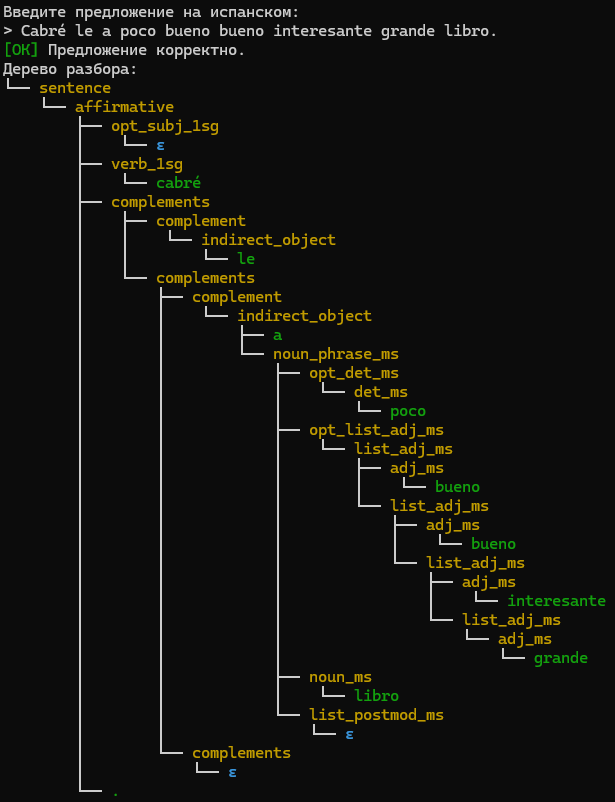
\includegraphics[width=1\linewidth]{image2a.png}
            \caption{\centeringСоответствующее предложение}
    \end{subfigure}
    \hfill % Распорка для равномерного распределения
    \begin{subfigure}[b]{0.45\textwidth}
            \centering
                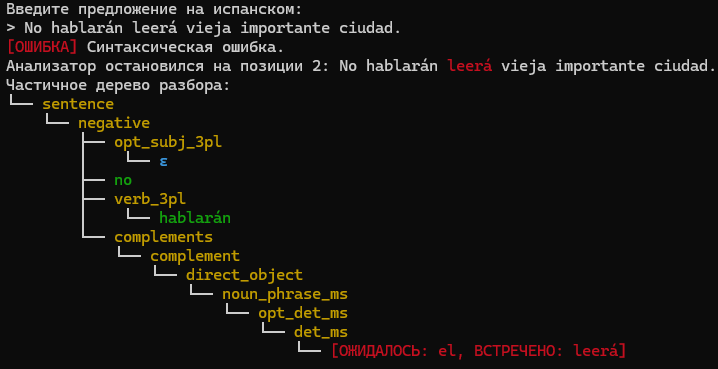
\includegraphics[width=1\linewidth]{image2b.png}
            \caption{\centeringНесоответствующее предложение}
    \end{subfigure}
    \caption{\centeringВывод программы при вводе предложения пользователем}
    \label{fig:both}
\end{figure}

Также на рисунке 4 представлен ввод пользователем корректного утвердительного, отрицательного и вопросительного предложений.
\begin{figure}[H]
    \centering
    
\includegraphics[width=0.75\linewidth]{image3.png}
    \caption{\centeringВвод утвердительного, отрицательного и вопросительного предложений}
\end{figure}

Далее на рисунках 5 и 6 представлена генерация предложений без вывода деревьев разбора 10 строк с 50\% некорректных строк и с 0\% соответственно.
\begin{figure}[H]
    \centering
    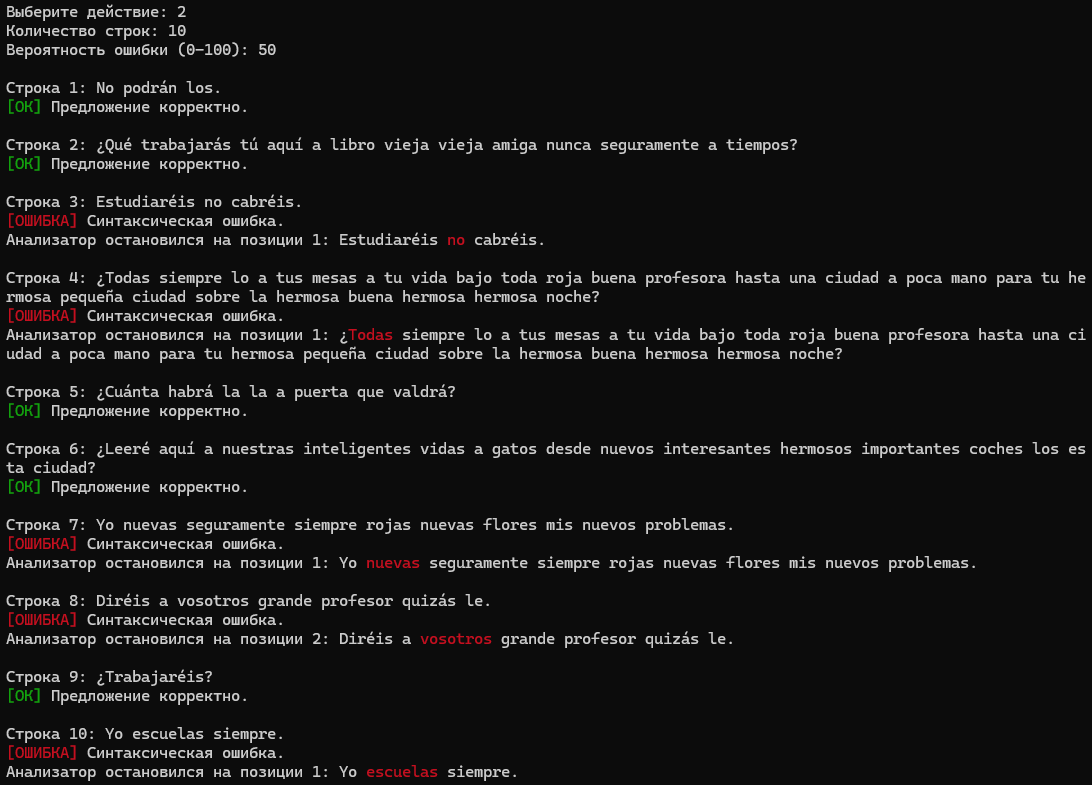
\includegraphics[width=0.75\linewidth]{image5.png}
    \caption{\centeringГенерация 10 предложений с 50\% некорректных}
\end{figure}


\begin{figure}[H]
    \centering
    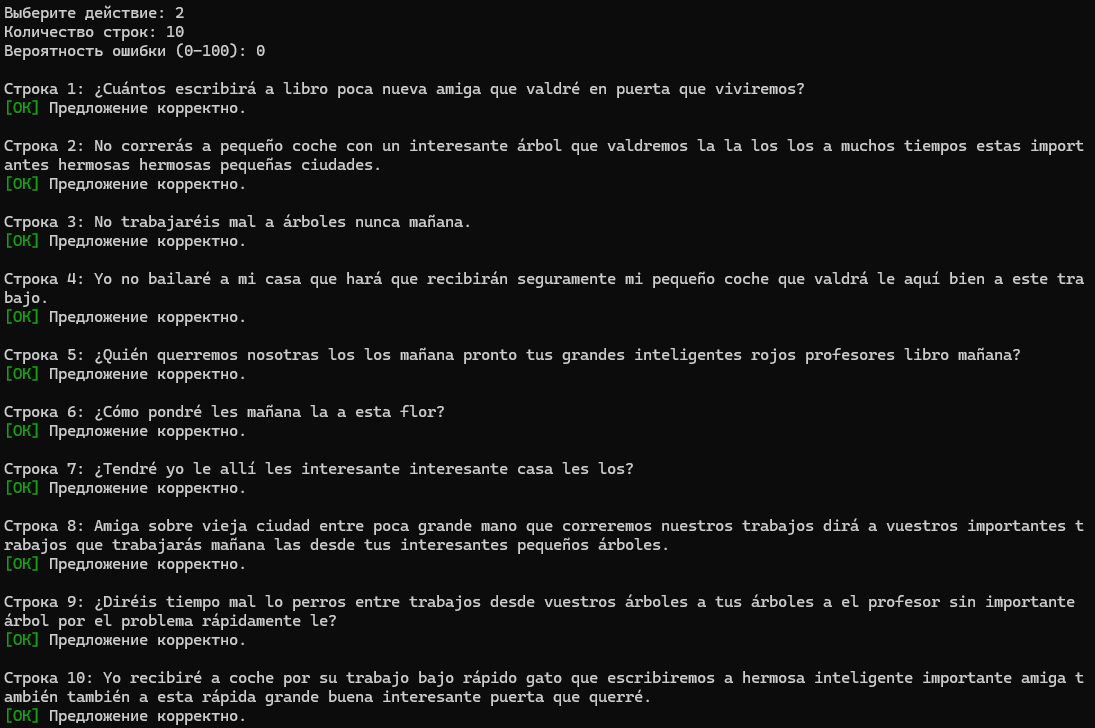
\includegraphics[width=0.75\linewidth]{image6.png}
    \caption{\centeringГенерация 10 предложений с 0\% некорректных}
\end{figure}


\newpage
\section*{Заключение}
\addcontentsline{toc}{section}{Заключение}
В ходе выполнения данной лабораторной работы была разработана контекстно-свободная грамматика для подмножества будущего простого времени испанского языка. 

Далее по данной грамматике были разработаны анализатор введённых пользователем предложений и генератор предложений, который поддерживает задание необходимого соотношения некорректных предложений к корректным.

Разработанная программа правильно обрабатывает и генерирует предложения из выбранного языка, а также может выводить дерево разбора предложения при работе с ним.

\textbf{Достоинства}:
\begin{itemize}
    \item Разработанный класс LanguageModel позволяет создавать анализаторы и генераторы любых КС грамматик.
    \item КС грамматики можно задавать с помощью простого перечисления правил вывода.
    \item Реализована генерации деревьев разбора предложений как при генерации, так и при валидации.
    \item При валидации и генерации предложений выводятся их деревья разбора. В случае, если предложение неправильное, также будет выводится одно из слов, которые программа ожидала встретить на позиции ошибочного слова.
\end{itemize}

\textbf{Недостатки}:
\begin{itemize}
    \item Для генерации и валидации предложений используется метод рекурсивного спуска с откатами, который выполняется с экспоненциальной сложностью по времени.
    \item При генерации предложений не учитывается их семантика из-за чего могут получаться семантически неправильные фразы.
\end{itemize}

\textbf{Масштабирование}:
\begin{itemize}
    \item Переписать класс грамматики так, чтобы внутри он хранил и использовал конечный автомат со стеком, представленный экземпляром класса FSM, разработанного в первой лабораторной работе.
\end{itemize}

\newpage
\addcontentsline{toc}{section}{Список использованной литературы}
\begin{thebibliography}{}
    \bibitem{litlink1} Секция <<Телематика>>.— Текст: электронный // tema.spbstu: [сайт].— URL: https://tema.spbstu.ru/mathem/ (дата обращения: 29.03.2026).
    \bibitem{litlink2} Вирт, Н. Построение компиляторов / Н. Вирт. – М.: ДМК Пресс, 2010. – 190 с.

    \bibitem{litlink3} Ахо, А. В. Компиляторы: принципы, технологии и инструментарий [2-е изд.] / А. В. Ахо, М. С. Лам, Р. Сети, Дж. Д. Ульман ; Пер. с англ. — М. : ООО «И.Д. Вильямс», 2018. — 1184 с.
\end{thebibliography}

\end{document}